\chapter{Contexto do Cliente}

\section{Empresa Júnior}

  Segundo Periard, empresa júnior é uma associação civil sem fins lucrativos que é
  composta por estudantes e que prestam serviço para diversos tipos de clientes em sua
  área de atuação, inclusive empresas de mercado, sob orientações de professores.\cite{periardej}

  No ano de 2016, sancionou-se a lei 13.267/16 que regulamenta a empresa júnior, impondo-se
  algumas restrições e direitos. A principal delas seria que uma empresa júnior não pode obter
  lucro para os membros, o dinheiro obtido com a prestação de serviços ou produtos são reinvestidos
  na própria empresa.

\section{Cráton}

  A Cráton é uma empresa júnior recente e formada por estudantes do curso de geologia da
  Universidade de Brasília que atualmente tem 15 membros. Possui uma hierarquia na qual o
  presidente está no topo, abaixo estão os diretores de cada setor da empresa, sendo os
  seguintes setores da Cráton:

  \begin{itemize}
    \item{Administrativo-Financeiro;}
    \item{Recursos Humanos;}
    \item{Projetos;}
    \item{Marketing;}
  \end{itemize}

  Em cada setor, existem dois assessores que à disposição dos diretores com os seguintes cargos:

  \begin{itemize}
    \item \textbf{Administrativo-Financeiro}: Assessoria de administração e assessoria
    e assesoria de finanças;
    \item \textbf{Recursos Humanos}: Assessoria de desenvolvimento e assessoria de implementação
    de práticas;
    \item \textbf{Projetos}: Assessoria de projeto interno e assessoria de projeto externo;
    \item \textbf{Marketing}: Assessoria de comunicação e assessoria de atendimento.
  \end{itemize}

  O organograma clássico, porém invertido seguinte contém a hierarquia da empresa, começando
  de baixo para cima:

  \begin{figure}[!ht]
    \centering
    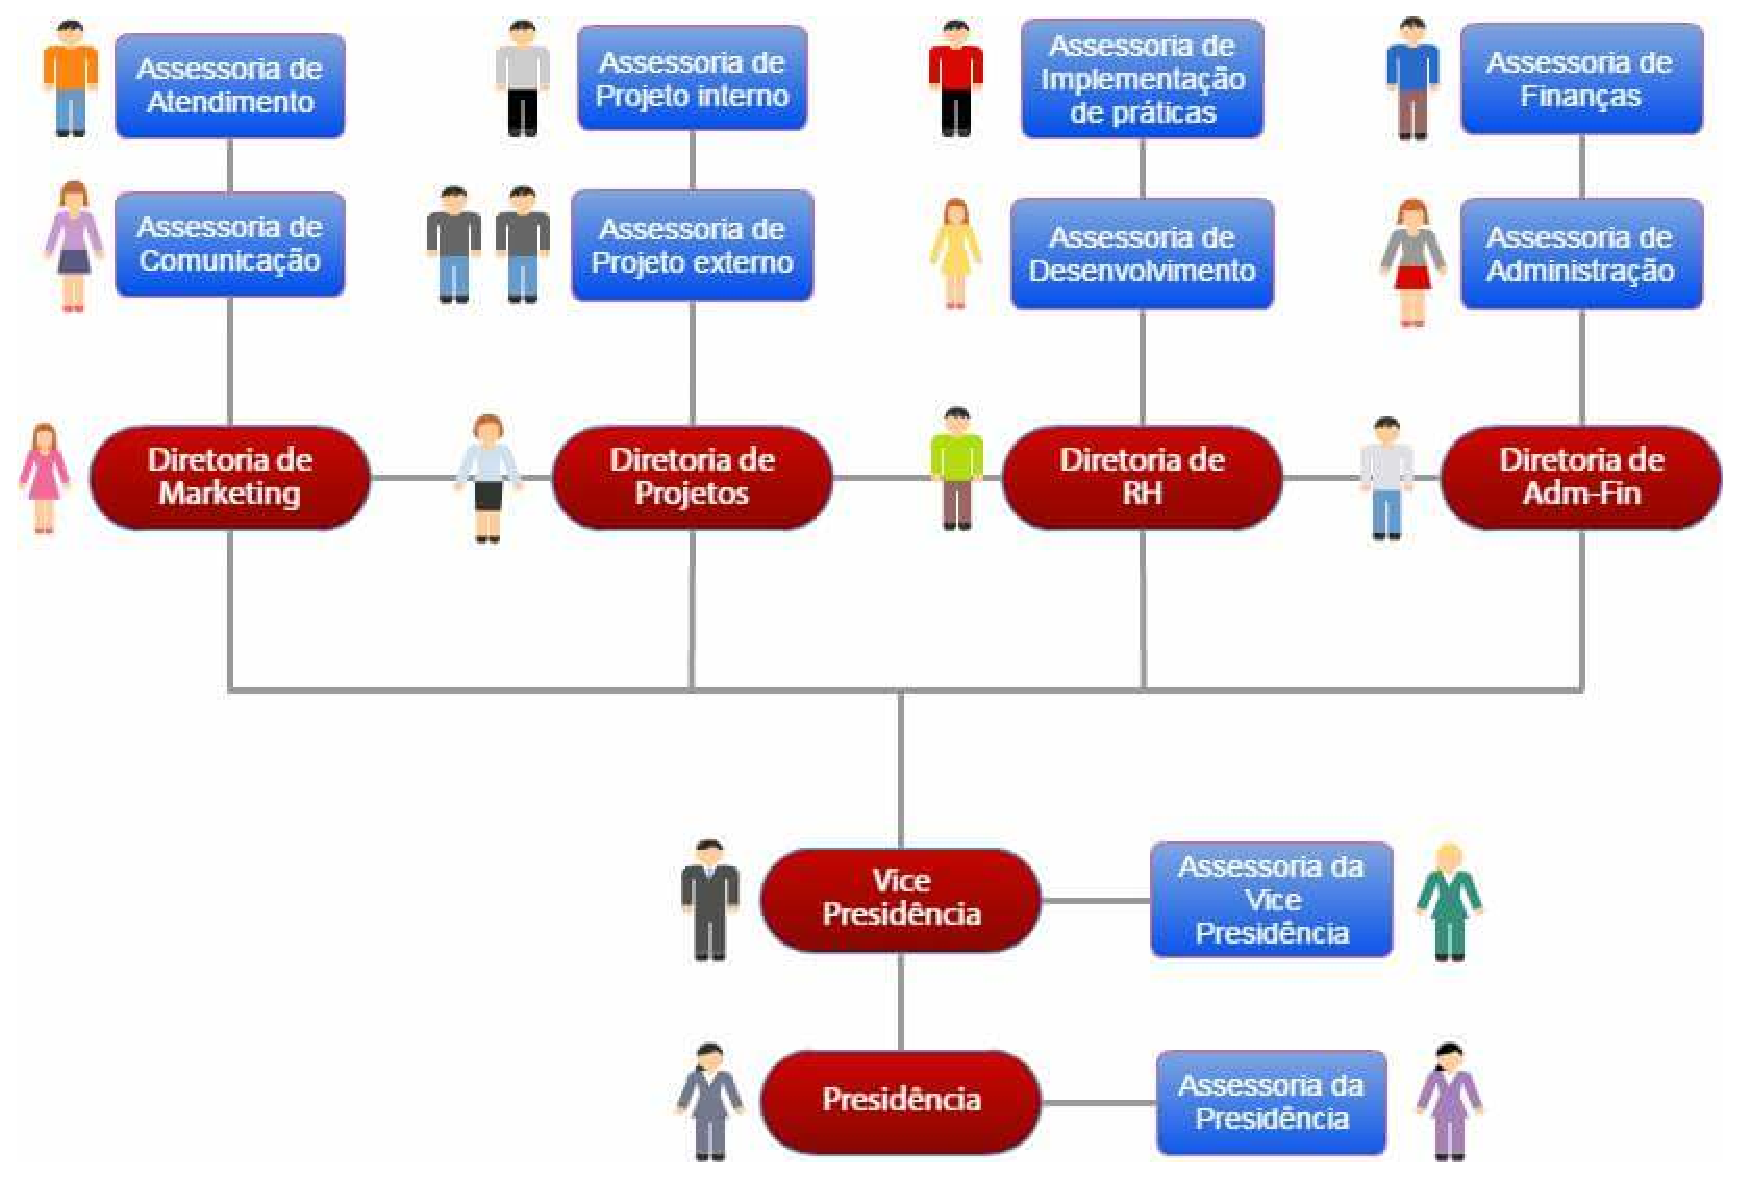
\includegraphics[width=15cm, keepaspectratio=true]{figuras/empresa/hierarquia-craton.eps}
    \caption{Hierarquia da Cráton}
  \end{figure}

  Além dos cargos inerentes aos membros da empresa, existem também os \textbf{colaboradores}
  que são pessoas que não participam com algum cargo direto na empresa, mas de alguma forma
  a auxilia.

  A empresa tem o objetivo de prestar serviços geológicos, sendo que os atuais produtos são
  de geoprocessamento e geologia de prospecção. Futuramente a Cráton pretende expandir a
  variedade de seus produtos abrangendo as áreas de espeleologia, geologia ambiental e
  geoturismo.

